\bookchapter{Chapter 42: LLM Landscape and API Practice}

\chapterintro{Previous chapters covered how to work with AI. This one answers a more basic question: which AI, and how? By August 2026 the LLM landscape is rich — globally GPT, Claude, and Gemini compete; in China DeepSeek, Tongyi Qianwen, GLM, Kimi, and Doubao bloom. Each model has its own personality and strengths: pick right and you fly; pick wrong and you drag. This chapter introduces the models, shows how to wire them into your apps via API, and how to choose a Token Plan that fits your usage.}

\booksection{Global major LLMs: the big three}

As of August 2026, the international LLM market is a three-way race: OpenAI (GPT), Anthropic (Claude), and Google (Gemini). Each has a distinct personality — let's meet them one by one.

\booksubsection{OpenAI GPT-5.6 series: the all-rounder}

OpenAI kicked off the LLM wave, and GPT remains the world's most widely used model family. The GPT-5.6 series, released July 2026, comes in three tiers: flagship GPT-5.6 Sol for high-end reasoning, balanced GPT-5.6 Terra for daily development, and lightweight GPT-5.6 Luna for high-throughput, low-cost scenarios. All three share a 1.05 million-token context window and support image input, function calling, and structured output.

\begin{center}
\begin{tabularx}{\linewidth}{|X|X|X|X|X|}
\hline
\textbf{Model} & \textbf{Positioning} & \textbf{Input (/1M tokens)} & \textbf{Output (/1M tokens)} & \textbf{Context window} \tabularnewline
\hline
GPT-5.6 Sol & Flagship reasoning & US\$5.00 (about ¥36) & US\$30.00 (about ¥217) & 1.05M tokens \tabularnewline
GPT-5.6 Terra & Balanced daily & US\$2.50 (about ¥18) & US\$15.00 (about ¥109) & 1.05M tokens \tabularnewline
GPT-5.6 Luna & Lightweight, low cost & US\$1.00 (about ¥7) & US\$6.00 (about ¥44) & 1.05M tokens \tabularnewline
\hline
\end{tabularx}
\end{center}

\begin{center}\small\color{gray}OpenAI GPT-5.6 series pricing (August 2026)\end{center}

GPT's core strength is balance — reasoning, coding, writing, multimodal, no glaring weaknesses. Plus OpenAI's huge plugin ecosystem and developer community, with the most complete docs and tooling. When you don't know what to pick, GPT is the safe default. Weak spots: needs special network access in China, occasional translation-flavored Chinese, and mid-to-high API prices.

\textbf{Good news}\par

In August 2026 OpenAI upgraded free users' default model to GPT-5.6 Luna and opened unlimited text chat. That means you can try GPT's basics at zero cost and only pay when you need stronger reasoning or API calls.

\booksubsection{Anthropic Claude series: coding and rigor at the top}

If GPT is the all-rounder, Claude is the coding ceiling. Anthropic's Claude series has long led SWE-bench (software engineering benchmark) by a wide margin, with top code quality and real-world engineering delivery. Even better, Claude's hallucination rate (chance of making things up) is the lowest online at about 1\% — ideal for academic, legal, and other high-precision work.

Claude's other killer feature is long context: up to 1 million tokens, able to “read” hundreds of pages of contracts or a whole codebase without missing details. Nearly irreplaceable for refactors and long-document analysis. Claude Code, the terminal AI coding tool, hit \$2.5 billion annualized revenue by mid-2026 — strong evidence of Claude's coding reputation.

\begin{center}
\begin{tabularx}{\linewidth}{|X|X|X|X|X|}
\hline
\textbf{Model} & \textbf{Positioning} & \textbf{Input (/1M tokens)} & \textbf{Output (/1M tokens)} & \textbf{Context window} \tabularnewline
\hline
Claude Fable 5 & Flagship & US\$10.00 (about ¥72) & US\$50.00 (about ¥362) & 1M tokens \tabularnewline
Claude Opus 4.8 & Professional & US\$5.00 (about ¥36) & US\$25.00 (about ¥181) & 1M tokens \tabularnewline
Claude Sonnet 5 & Value & US\$2.00 (about ¥14) & US\$10.00 (about ¥72) & 1M tokens \tabularnewline
\hline
\end{tabularx}
\end{center}

\begin{center}\small\color{gray}Anthropic Claude series pricing (August 2026; Sonnet 5 at promotional rate)\end{center}

Claude's downside is price — Fable 5 output is the most expensive of all models at \$50 per million tokens. Multimodal (image/video understanding) is also relatively weak. For individual developers on a budget, Sonnet 5's promotional price is excellent value.

\booksubsection{Google Gemini series: the multimodal king}

Google's Gemini series reached 3.1 Pro in 2026. Its biggest edge is native multimodal — precise image-text parsing, accurate OCR for tables, efficient video frame extraction, and deep audio/video analysis. Deeply tied to Google's ecosystem (Search, Gmail, cloud), it shines at real-time information retrieval and cross-modal understanding. Gemini also supports up to 2 million tokens of context — the largest window today.

Gemini positions itself as the first choice for scientific reasoning and multimodal work. If your project involves lots of image analysis, video understanding, or scientific computing, Gemini has few rivals. But pure-text code generation is slightly behind Claude, and its Chinese is less natural than domestic models.

\begin{center}
\begin{tabularx}{\linewidth}{|X|X|X|X|}
\hline
\textbf{Comparison item} & \textbf{GPT-5.6} & \textbf{Claude Fable 5} & \textbf{Gemini 3.1 Pro} \tabularnewline
\hline
Overall score & 94.8 & 95.0 & 92.1 \tabularnewline
Coding (SWE-bench) & 74.9\% & 64.3\% (Pro) & Medium \tabularnewline
Context window & 1.05M tokens & 1M tokens & 2M tokens \tabularnewline
Multimodal & Balanced & Weaker & Strongest \tabularnewline
Hallucination rate & Relatively low & Lowest (\textasciitilde{}1\%) & Relatively low \tabularnewline
Availability in China & Needs special network & Needs special network & Needs special network \tabularnewline
API ecosystem & Most complete & Growing & Tied to Google ecosystem \tabularnewline
\hline
\end{tabularx}
\end{center}

\begin{center}\small\color{gray}Side-by-Side Comparison of the Big Three International Models (August 2026)\end{center}

\begin{tcbwarn}{Note: Real-World Hurdles for Users in China}
For developers in China, the core obstacle to GPT, Claude, and Gemini is network access. You can reach them indirectly through Azure proxies, API aggregation platforms, and the like, but you'll need to weigh stability and compliance yourself. If your project has strict data security requirements, we recommend looking at Chinese models first.

\end{tcbwarn}

\booksection{China's Major Large Models: A Hundred Flowers in Bloom}

By 2026, China's large models have gone from 'chasers' to running neck and neck with the leaders, and in some areas they have even pulled ahead. Unlike the 'wrapper' controversies of 2023, the flagship Chinese models of 2026 are on par with top international models in logical reasoning, code generation, and Chinese-language understanding, with the gap narrowed to within 5\%. More importantly, Chinese models have irreplaceable advantages in Chinese-language scenarios, cost, and compliant deployment.

\booksubsection{DeepSeek V4: The Best Bang for Your Buck}

DeepSeek is a phenomenon among Chinese large models. In early 2025, DeepSeek-V3 shook the market with its positioning of 'one-tenth the price of GPT with comparable capability,' and the industry dubbed it the 'kill line' for general-purpose AI models — nothing cheaper works as well, and nothing more expensive gives you more. By August 2026, DeepSeek V4-Pro was officially released: a 1.6-trillion-parameter MoE architecture with about 49B parameters active, support for 1 million tokens of lossless context, and coding value widely seen as the best in the world.

DeepSeek V4 made a huge leap in agent capability — its DeepSWE benchmark score jumped from 12.8 to 62.7 (+390\%), and NL2Repo rose from 38.5 to 61.5. The API now supports both the Responses API and the Anthropic API, so it works with mainstream coding tools like Codex and Claude Code. That means you can swap DeepSeek's API in for Claude's and use it inside Claude Code — cutting your costs several times over with a nearly identical experience.

\begin{center}
\begin{tabularx}{\linewidth}{|X|X|X|X|X|}
\hline
\textbf{Model} & \textbf{Positioning} & \textbf{Input (per 1M tokens)} & \textbf{Output (per 1M tokens)} & \textbf{Context Window} \tabularnewline
\hline
DeepSeek V4 Pro & Flagship reasoning & 3 yuan (approx. US\$0.43) & 6 yuan (approx. US\$0.87) & 1M tokens \tabularnewline
DeepSeek V4 Flash & Lightweight and fast & 1 yuan (approx. US\$0.14) & 2 yuan (approx. US\$0.28) & 1M tokens \tabularnewline
\hline
\end{tabularx}
\end{center}

\begin{center}\small\color{gray}DeepSeek V4 series pricing (August 2026, promotional prices)\end{center}

Price comparison: for the same 1 million input tokens plus 1 million output tokens, DeepSeek V4 Flash costs about \$0.42, GPT-5.6 Sol costs about \$35, and Claude Fable 5 costs about \$60. That is a gap of 80 to 140 times.

\textbf{Watch Out: DeepSeek Is About to Raise Its Prices}\par

On August 6, 2026, DeepSeek officially announced that it 'plans to significantly raise API prices in the near future,' so the promotional prices may not last long. Some media reports speculate the increase could be as much as 30 times, and as of August 14 the company had not yet published its final pricing plan. On top of that, the official DeepSeek V4 release introduced peak/off-peak pricing — calls during peak hours cost exactly double. Keep an eye on the official announcements for the latest prices.

\booksubsection{Tongyi Qianwen Qwen3.7 Max: Alibaba Cloud's Enterprise Choice}

Alibaba Cloud's Qwen (Tongyi Qianwen) series leans on the Alibaba Cloud ecosystem, giving it a natural edge in enterprise deployment. Qwen3.7 Max, released in July 2026, is the current flagship: a dense 235B-parameter model with 256K of native context, expandable to 1M. Qwen's core strengths are a mature open-source ecosystem (the entire lineup from 7B to 235B is open source), precise understanding of Chinese-language scenarios, and deep integration with Alibaba Cloud infrastructure.

\begin{center}
\begin{tabularx}{\linewidth}{|X|X|X|}
\hline
\textbf{Model} & \textbf{Output Price (per 1M tokens)} & \textbf{Use Case} \tabularnewline
\hline
qwen-turbo & 0.6 yuan & Simple Q\&A, text classification, high concurrency \tabularnewline
qwen-long & 2.0 yuan & 10M ultra-long context processing \tabularnewline
qwen3.7-flash & 7.2 yuan & General conversation, content generation \tabularnewline
qwen3.7-plus & 12.0 yuan & Multimodal (images + video), Chinese content creation \tabularnewline
qwen3.7-max & 36.0 yuan & Flagship Chinese capability, complex tasks \tabularnewline
\hline
\end{tabularx}
\end{center}

\begin{center}\small\color{gray}Qwen (Tongyi Qianwen) series tiered pricing (August 2026)\end{center}

Qwen's pricing is tiered — from the ultra-low-cost qwen-turbo (0.6 yuan per 1M output tokens) up to the flagship qwen3.7-max (36 yuan per 1M output tokens), covering everything from lightweight Q\&A to complex reasoning. For companies already on Alibaba Cloud, Qwen is the most convenient integration choice.

\booksubsection{Zhipu GLM-5.1: Top Chinese Model on SWE-bench}

Zhipu AI's GLM series shone in 2026. GLM-5.1 took first place among Chinese models on SWE-bench: a 744B hybrid MoE-dense architecture with support for 1 million tokens of context. Its hallmarks are precise Chinese semantic understanding and support for compliant private deployment in China — which matters a great deal for finance and government scenarios with strict data security requirements. GLM-5.1 is priced at 6 yuan for input and 24 yuan for output per 1M tokens, in the middle of the pack among Chinese models.

\booksubsection{Kimi K3: The King of Ultra-Long Text}

Moonshot AI's Kimi series is known for its ultra-long text handling. Kimi K3, released in July 2026, has 2.8 trillion parameters and lands in the global top tier across many complex-task benchmarks. Kimi's core use cases are large codebase analysis and long-document retrieval augmentation — it can chew through the text of an entire book or the code of an entire project, and it excels at 'needle in a haystack' retrieval tasks. Kimi is relatively pricey (about 12-20 yuan per 1M output tokens), but in long-text scenarios nothing else matches its value for money.

\booksubsection{Doubao: ByteDance's All-Rounder}

ByteDance's Doubao series has been steady in 2026. Doubao Seed 2.1 Pro is the flagship model on Volcano Engine, with 256K context and consistently solid results in real-world testing, standing out in Chinese-language scenarios. Doubao's advantages: a big bundle of free tokens the moment you register, well-polished integration with the Volcano Engine ecosystem, and pricing among the lowest tiers in China. For beginners who want a quick taste of AI coding, Doubao is a zero-barrier way in.

\begin{center}
\begin{tabularx}{\linewidth}{|X|X|X|X|X|X|}
\hline
\textbf{Comparison Item} & \textbf{DeepSeek V4} & \textbf{Qwen3.7 Max} & \textbf{GLM-5.1} & \textbf{Kimi K3} & \textbf{Doubao 2.1 Pro} \tabularnewline
\hline
Overall Score & 87.5 & 89.7 & 90.5 & 88+ & 85+ \tabularnewline
Coding Ability & Extremely strong & Strong & No. 1 in China on SWE & Strong & Above average \tabularnewline
Chinese Understanding & Excellent & Excellent & Precise & Excellent & Excellent \tabularnewline
Context Window & 1M & 256K-1M & 1M & Ultra-long & 256K \tabularnewline
Output Price (yuan per 1M) & 6 & 36 & 24 & 12-20 & 30 \tabularnewline
Open Source & MIT license & Entire lineup open source & Partially open source & Closed source & Closed source \tabularnewline
Private Deployment & Yes & Yes & Yes & No & No \tabularnewline
\hline
\end{tabularx}
\end{center}

\begin{center}\small\color{gray}Side-by-Side Comparison of China's Top Five Models (August 2026)\end{center}

One important trend: the sense of a 'generation gap' between Chinese models and GPT/Claude has disappeared. In logical reasoning and math competitions, Chinese flagships trail GPT-5 by single digits. Claude still leads in systematic architectural thinking and complex engineering reasoning — it produces architecture plans with more 'flair,' while Chinese models can sometimes come across as 'by the book.' But in Chinese-language scenarios, cost control, and compliant deployment, Chinese models hold an overwhelming advantage.

\begin{center}
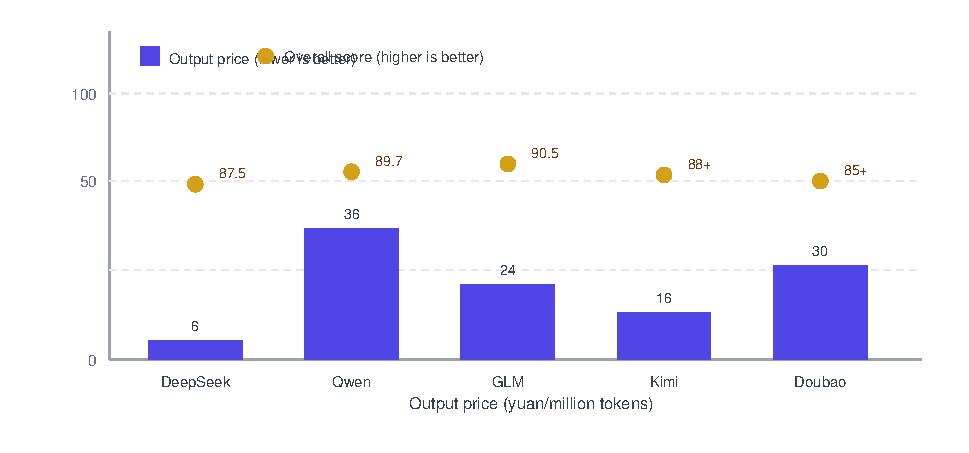
\includegraphics[width=0.92\linewidth]{figures/fig-di-si-shi-er-zhang-1}
\\[2pt]\small Figure 4: Price vs. Performance of the Five Models (lower price is better, higher score is better)
\end{center}

\booksection{A Decision Framework for Choosing a Model}

Now that you know each model's strengths, how do you pick one for your project? Here is a 'four-question decision method' — answer four questions, and you'll lock onto the model that fits you best.

Is your project deployed in China or internationally?

China choose a Chinese model

|

International overseas models are an option

Is the core task coding or something else?

Coding Claude or DeepSeek

|

Other keep narrowing down

Need extra-long context (>500K tokens)?

Yes Gemini or Kimi

|

No keep narrowing down

Is budget a concern?

Yes DeepSeek or Qwen-turbo

|

No GPT-5.6 or Claude

\begin{center}\small\color{gray}Figure 5: The Four-Question Decision Method for Choosing a Large Model\end{center}

\begin{tcbinfo}{Tip: The Combination Strategy}
This decision method isn't dogma — many situations call for combining several models. One common strategy: use DeepSeek or Qwen for everyday development (cheap, good with Chinese), Claude for critical architecture design (strong reasoning, low hallucination), and Gemini for multimodal analysis (image and video processing). Switch models as needed instead of riding 'one model to the grave.'

\end{tcbinfo}

\booksection{Getting Started with API Calls: Connecting to a Large Model from Scratch}

Many AI coding tutorials only teach you how to use the chat interface, but real 'AI programming' — having your application call a large model — goes through an API. An API (Application Programming Interface) is a communication protocol between programs. Through an API, your code can call on a large model's abilities as easily as calling a function.

\booksubsection{What Is a Token}

Before APIs, you must first understand the concept of a 'token.' A token is the basic billing unit for large models — think of it as the AI's unit of reading and writing. One token is roughly 0.75 English words (4 characters), or 0.5-1 Chinese characters. A 1,000-character Chinese passage consumes about 1,500-2,000 tokens.

A token is not a word count, nor a character count. Large models use a dedicated tokenizer to split text into tokens. The same word can cost a different number of tokens in different models — 'artificial intelligence,' for instance, might be 3 tokens in GPT but 2 in DeepSeek. Most models' APIs return the actual number of tokens consumed, and you can check it in the API response.

\begin{tcbinfo}{Quick Token Cost Estimates}
One million Chinese characters is roughly 1.5 million tokens. Processing 1 million characters of input plus 1 million characters of output with DeepSeek V4 Flash costs about \$0.42 (around 3 yuan); the same volume with Claude Fable 5 costs about \$60 (around 434 yuan). That is why your choice of model directly shapes your project's cost.

\end{tcbinfo}

\booksubsection{Getting an API Key}

The first step in using a large model API is getting an API Key — a string used to verify your identity. Every model provider has its own API platform, where you register an account and create an API Key. Here are the API platform entry points for the mainstream models and the steps to get a key:

\begin{center}
\begin{tabularx}{\linewidth}{|X|X|X|X|}
\hline
\textbf{Model} & \textbf{API Platform} & \textbf{How to Get a Key} & \textbf{Free Allowance} \tabularnewline
\hline
DeepSeek & platform.deepseek.com & Sign up identity verification create API Key & Free allowance for new users \tabularnewline
Qwen (Tongyi Qianwen) & bailian.aliyun.com (Bailian platform) & Log in with an Alibaba Cloud account activate the service create a Key & Free trial for new users \tabularnewline
Zhipu GLM & open.bigmodel.cn & Sign up identity verification create API Key & Free allowance for new users \tabularnewline
Kimi & platform.moonshot.cn & Sign up identity verification create API Key & Limited free allowance \tabularnewline
Doubao & volcengine.com (Volcano Engine) & Sign up activate Volcano Ark create API Key & Large free token grant just for signing up \tabularnewline
OpenAI GPT & platform.openai.com & Sign up link a credit card create API Key & No free allowance (paid) \tabularnewline
Anthropic Claude & console.anthropic.com & Sign up link a card create API Key & Small allowance for new users \tabularnewline
\hline
\end{tabularx}
\end{center}

\begin{center}\small\color{gray}API platforms for mainstream models and how to get a key (August 2026)\end{center}

\textbf{Security Note: Your API Key Is Your Wallet Password}\par

An API Key is the equivalent of your wallet password — anyone who gets hold of it can spend your quota calling the model. So: never write an API Key into your code (manage it with environment variables); never commit code containing a Key to a public Git repository; never share screenshots containing a Key on social media. If a Key leaks, delete it on the platform and create a new one immediately.

\booksubsection{Your First API Call}

Once you have an API Key, you can call a large model API from any programming language. Here is the simplest possible call, shown in Python — send one message to DeepSeek and get the reply back.

\begin{lstlisting}[language=Python]
# Install the SDK: pip install openai
# DeepSeek is compatible with the OpenAI SDK format — use it directly
from openai import OpenAI
import os

# 1. Create the client (the API key is read from an environment variable)
client = OpenAI(
    api_key=os.environ.get("DEEPSEEK_API_KEY"),
    base_url="https://api.deepseek.com"
)

# 2. Send the request
response = client.chat.completions.create(
    model="deepseek-chat",  # pick the model
    messages=[
        {"role": "system", "content": "You are a Python coding assistant."},
        {"role": "user", "content": "Write a quicksort function."}
    ]
)

# 3. Get the reply
print(response.choices[0].message.content)

# 4. Check token usage
print(f"Input tokens: {response.usage.prompt_tokens}")
print(f"Output tokens: {response.usage.completion_tokens}")
print(f"Total tokens: {response.usage.total_tokens}")
\end{lstlisting}

The core logic of this code: create a client (carrying the API Key and the model address) build the message list (system sets the role, user is the human's input) send the request get the reply. This pattern works for nearly every OpenAI-compatible model — just swap the api\_key and base\_url to change models. That is why so many Chinese models choose to be OpenAI SDK compatible: developers can switch models by changing two lines of code, so the cost of migrating is almost nil.

Here is what changes when you switch to another model — note that only two lines need to change:

\begin{lstlisting}[language=Python]
# DeepSeek
client = OpenAI(
    api_key=os.environ.get("DEEPSEEK_API_KEY"),
    base_url="https://api.deepseek.com"
)
# model="deepseek-chat"

# Qwen (Tongyi Qianwen, Bailian platform)
client = OpenAI(
    api_key=os.environ.get("DASHSCOPE_API_KEY"),
    base_url="https://dashscope.aliyuncs.com/compatible-mode/v1"
)
# model="qwen-plus"

# Zhipu GLM
client = OpenAI(
    api_key=os.environ.get("GLM_API_KEY"),
    base_url="https://open.bigmodel.cn/api/paas/v4"
)
# model="glm-4"

# OpenAI GPT
client = OpenAI(
    api_key=os.environ.get("OPENAI_API_KEY"),
    # the default base_url is fine
)
# model="gpt-5.6-terra"
\end{lstlisting}

\booksubsection{Streaming Responses}

In a real application, you usually don't want to wait for the AI to finish everything before displaying it in one lump — that makes users wait far too long. Streaming responses let the text appear word by word as the AI generates it, which vastly improves the user experience. Like a typewriter with letters popping out one at a time — it feels completely different to the user.

\begin{lstlisting}[language=Python]
# Streaming: output one character at a time
stream = client.chat.completions.create(
    model="deepseek-chat",
    messages=[
        {"role": "user", "content": "Write a tutorial on bubble sort in Python"}
    ],
    stream=True  # enable streaming
)

# Receive chunk by chunk and print
for chunk in stream:
    if chunk.choices[0].delta.content is not None:
        print(chunk.choices[0].delta.content, end="", flush=True)
# The output appears character by character, like a typewriter
\end{lstlisting}

\booksection{A Buyer's Guide to Token Plans}

Most model providers offer two billing methods: pay-as-you-go and subscription plans (Token Plans). Understanding the difference between the two can cut your costs dramatically.

\booksubsection{Pay-As-You-Go vs. Subscription Plans}

\begin{center}
\begin{tabularx}{\linewidth}{|X|X|X|}
\hline
\textbf{Aspect} & \textbf{Pay-as-you-go} & \textbf{Subscription plan} \tabularnewline
\hline
Billing Method & Pay only for the tokens you use & Pay a fixed amount up front and receive an allowance \tabularnewline
Best For & Unsteady usage, occasional calls & Steady usage, frequent calls \tabularnewline
Price Advantage & Standard price & 20\%-50\% cheaper than pay-as-you-go \tabularnewline
Flexibility & Available anytime, no commitment & Requires prepayment; unused allowance may expire \tabularnewline
Going Over Quota & Automatically billed as you go & Switches to pay-as-you-go once the allowance runs out \tabularnewline
Typical Platforms & Each model's official API platform & OpenAI Plus/Pro, Claude Pro, Cursor Pro \tabularnewline
\hline
\end{tabularx}
\end{center}

\begin{center}\small\color{gray}Comparing the Two Billing Methods\end{center}

For beginners, start with pay-as-you-go — no upfront cost, and you pay for exactly what you use. Once your monthly usage settles at a steady level (say, above 50 yuan a month), consider switching to a subscription plan for a lower unit price.

\booksubsection{Mainstream Subscription Plans at a Glance}

\begin{center}
\begin{tabularx}{\linewidth}{|X|X|X|X|}
\hline
\textbf{Plan} & \textbf{Monthly Fee} & \textbf{What's Included} & \textbf{Best For} \tabularnewline
\hline
ChatGPT Free & Free & Unlimited text chat with GPT-5.6 Luna & Trying it out as a total beginner \tabularnewline
ChatGPT Plus & US\$20/month & GPT-5.6 Sol, image generation, data analysis, plugin access & Moderate users \tabularnewline
ChatGPT Pro & US\$200/month & Unlimited use of all models, priority access to new features & Heavy professional users \tabularnewline
Claude Free & Free & A limited number of Claude chats & Trying it out as a total beginner \tabularnewline
Claude Pro & US\$20/month & Unlimited Claude usage, priority access to new models & Coders \tabularnewline
Cursor Free & Free & A limited number of AI completions and chats & Getting started as a beginner \tabularnewline
Cursor Pro & US\$20/month & Unlimited AI completions, 500 premium requests per month & Everyday developers \tabularnewline
Cursor Business & US\$40/month per person & Team collaboration, admin console, privacy mode & Teams \tabularnewline
\hline
\end{tabularx}
\end{center}

\begin{center}\small\color{gray}Mainstream AI tool subscription plans (August 2026)\end{center}

Chinese models handle subscriptions a little differently. DeepSeek is mainly pay-as-you-go, with no monthly subscription plan — you top up and get charged based on actual usage. Qwen offers prepaid resource packages on the Bailian platform (buy a fixed amount of tokens at a discounted price). Doubao has similar prepaid options on Volcano Engine. For developers in China, the most economical combination is usually: DeepSeek pay-as-you-go (daily development) plus Doubao's free allowance (trying things out).

\booksubsection{API Aggregation Platforms}

If you need to use several models at once, an API aggregation platform is a hassle-free option. An aggregator gives you one unified API Key that can call dozens of models worldwide, with no need to register separately on each platform.

\begin{center}
\begin{tabularx}{\linewidth}{|X|X|X|X|}
\hline
\textbf{Platform} & \textbf{Features} & \textbf{Price Advantage} & \textbf{Best For} \tabularnewline
\hline
OpenRouter (openrouter.ai) & Overseas aggregator: one Key for models worldwide & Transparent pricing with real-time comparison & Flexibly switching among many overseas models \tabularnewline
SiliconFlow (siliconflow.cn) & China-based aggregator offering APIs for many Chinese models & 20\%-30\% below official prices & Developers in China comparing model prices \tabularnewline
Azure OpenAI (Microsoft's proxy) & The OpenAI API proxied through Microsoft Azure & 50\% off with the Batch API & Enterprise-grade OpenAI calls; large asynchronous batches \tabularnewline
Baidu Qianfan (qianfan.baidubce.com) & Baidu's AI cloud platform, offering ERNIE and other models & Free allowance for new users & Users in Baidu's ecosystem \tabularnewline
\hline
\end{tabularx}
\end{center}

\begin{center}\small\color{gray}Mainstream API Aggregation Platforms (August 2026)\end{center}

\textbf{Watch Out: Don't Buy 'Shared Keys'}\par

Do not buy so-called 'shared API Keys' on Taobao, Xianyu, or similar platforms — these Keys usually come from unclear sources, can be banned at any moment, and carry the risk of data leaks. Always get API Keys through official platforms or reputable aggregators.

\booksubsection{Cost Optimization Strategies}

Picking the right model is only the first step — knowing how to 'use it frugally' matters just as much. Here are a few cost optimization strategies proven in practice:

\begin{enumerate}
  \item Make the most of cache hits. Many models offer 'caching' — when your request includes content that has been processed before (such as a system prompt), that portion is billed at a tiny fraction of the normal price. DeepSeek charges just 1/60 of the regular price for cache hits. Putting your fixed system prompt at the start of the message list maximizes cache hits.
  \item Tiered routing — use a cheap model for simple tasks and an expensive one for complex tasks. For example, DeepSeek V4 Flash for text classification (2 yuan per 1M output tokens) and Claude for architecture design (181 yuan per 1M output tokens). In a typical project, 80\% of calls can go to the cheap model.
  \item Cap your output length. APIs bill by output tokens, so longer output costs more. In scenarios that don't call for long-winded answers, set the max\_tokens parameter to limit output length and keep the AI from 'rambling on.'
  \item Use the Batch API for non-real-time tasks. If you have lots of tasks that don't need instant responses (such as bulk data labeling or document summarization), the Batch API earns you a 50\% discount. Both OpenAI and Azure offer this feature.
  \item Monitor your token usage. Most API platforms provide a usage dashboard. Check the usage breakdown regularly, find the calls that burn the most tokens, and optimize them specifically. One small prompt tweak (say, changing 'please explain in detail' to 'please explain in 3 sentences') can save 50\% of your tokens.
\end{enumerate}

\begin{center}
\begin{tabularx}{\linewidth}{|X|X|X|X|}
\hline
\textbf{Strategy} & \textbf{Savings} & \textbf{Difficulty} & \textbf{Notes} \tabularnewline
\hline
Cache hits & Up to 98\% & Low & Put fixed content at the start of your messages \tabularnewline
Tiered routing & 50\%-80\% & Mid & Use a cheap model for simple tasks \tabularnewline
Cap output length & 30\%-60\% & Low & Set the max\_tokens parameter \tabularnewline
Batch API & 50\% & Low & Use batch processing for non-real-time tasks \tabularnewline
Prompt optimization & 20\%-50\% & Mid & Streamline prompts and trim redundancy \tabularnewline
\hline
\end{tabularx}
\end{center}

\begin{center}\small\color{gray}Cost optimization strategies and their impact (August 2026)\end{center}

\booksection{Hands-On: Wiring a Large Model API into a Project}

Let's wrap up the chapter with a complete hands-on exercise — building an 'AI Summarizer': the user pastes in a long piece of text, and the app calls a large model API to produce a summary. This exercise walks through the full API workflow: environment setup, the API call, error handling, and cost control.

\begin{lstlisting}[language=Python]
# ai_summarizer.py - AI summarizer
import os
from openai import OpenAI

# 1. Configure (the API key is read from an environment variable — never hard-code it)
client = OpenAI(
    api_key=os.environ.get("DEEPSEEK_API_KEY"),
    base_url="https://api.deepseek.com"
)

def summarize(text: str, max_length: int = 200) -> dict:
    """Summarize a text

    Args:
        text: the original text to summarize
        max_length: maximum summary length (in tokens)

    Returns:
        dict: the summary plus token-usage info
    """
    try:
        response = client.chat.completions.create(
            model="deepseek-chat",
            messages=[
                {
                    "role": "system",
                    "content": "You are a summarizer."
                               "Summarize the user's text concisely."
                               "Keep the summary to 3 sentences at most."
                },
                {
                    "role": "user",
                    "content": f"Summarize the following text:\n\n{text}"
                }
            ],
            max_tokens=max_length,  # cap the output length
            temperature=0.3  # low temperature = more stable
        )

        return {
            "success": True,
            "summary": response.choices[0].message.content,
            "input_tokens": response.usage.prompt_tokens,
            "output_tokens": response.usage.completion_tokens,
            "total_tokens": response.usage.total_tokens
        }

    except Exception as e:
        return {
            "success": False,
            "error": str(e)
        }

# 2. Usage example
if __name__ == "__main__":
    long_text = """
    (paste a long text here...)
    """

    result = summarize(long_text)

    if result["success"]:
        print(f"Summary: {result['summary']}")
        print(f"Tokens used: {result['total_tokens']}")
        # estimate the cost: DeepSeek V4 Flash
        cost = result['total_tokens'] * 0.000004  # about 0.4 fen per 1,000 tokens
        print(f"Estimated cost: {cost:.4f} yuan")
    else:
        print(f"Something went wrong: {result['error']}")
\end{lstlisting}

This code embodies several API best practices: the API Key is read from an environment variable and never hardcoded; the function has clear documentation and type hints; max\_tokens is set to cap the output length; temperature is set low (0.3) for more stable output; error handling is complete; and token consumption is returned for cost tracking. When you have the AI write this code, you can simply tell it these requirements — it is fully capable of implementing them.

The final lesson of this chapter: models are the "ammunition," methodology is the "tactics." The right ammunition makes the battle smoother, but without good tactics even the best ammo loses the war. Now that you know each model's strengths and how to use the APIs, you have a well-stocked arsenal — but how you fight the battle still depends on the thinking methods from the earlier chapters.

\begin{tcbpractice}{Try It Yourself: Get Your First API Call Running}
Register on a Chinese model platform (we recommend DeepSeek or Zhipu — both give new users a free allowance), create an API Key, put it into your system environment variables (not into your code!), and then run the 'first API call' code above. The moment you see the AI's reply print out, you have crossed the line between 'using AI' and 'building AI applications.'

\end{tcbpractice}

\begin{tcbsummary}{Chapter Recap}
\begin{itemize}
  \item The big three international models: GPT-5.6 (a balanced all-rounder), Claude (top-tier coding with a hallucination rate of just 1\%), Gemini (king of multimodal with 2M context)
  \item China's top five: DeepSeek V4 (best value for money — watch for the price-increase announcement), Qwen3.7 (enterprise-grade), GLM-5.1 (No. 1 in China on SWE), Kimi K3 (ultra-long text), Doubao (a free way to start)
  \item The four-question decision method: Where will it be deployed? Coding or something else? Ultra-long context? Tight budget?
  \item Tokens are the billing unit: 1 Chinese character is about 1.5-2 tokens; 1 million characters is about 1.5 million tokens
  \item An API Key is your wallet password: manage it with environment variables, never hardcode it, never upload it to Git
  \item Chinese models are generally OpenAI SDK compatible: switching models means changing just two lines — api\_key and base\_url
  \item Five ways to save: cache hits, tiered routing, capping output, the Batch API, and monitoring usage
\end{itemize}

\end{tcbsummary}
